\section{Derivatives computation}

Computation of derivative quantities such as gradient and Laplacian is of fundamental importance in
data analysis. In this section, we studies streams that aim to minimize errors of derivative fields.
For the experiments in this section, we quantize the data to $32$ instead of $16$ bits, to ensure
enough precision for the purpose of computing derivatives.

\subsection{Gradient}

% Since simulation data can rarely be captured by closed-form formulas, we use finite difference to
% compute gradients. We experiment with three popular finite difference schemes using stencil sizes of
% two, three, and five points, to compute partial derivatives in each direction: $\frac{\partial
% f}{\partial x}\approx f(x+1)-f(x) \approx \frac{1}{2}f(x+1)-\frac{1}{2}f(x-1) \approx
% \frac{1}{12}f(x-2)-\frac{2}{3}f(x-1)+\frac{2}{3}f(x+1)-\frac{1}{12}f(x+2)$. The gradient at each
% grid point $(x,y)$ is the vector $(\frac{\partial f}{\partial x},\frac{\partial f}{\partial y})$. We
% use the greedy algorithm in Section (\Cref{sec:data_dep_streams} to compute a stream that minimizes
% the difference between the gradient field of $f_b$ (the reconstructed function using $b$ bits per
% sample) and that of the original function ($f$). At each grid point $p$, we compute an error $e(p)$,
% defined to be the squared Euclidean length of the difference between two gradient vectors at $p$,
% that is $e(p)=\norm{\nabla f_b(p)-\nabla f(p)}^2$. The overall error metric, $E_g$, over the whole
% field is defined as $E_g(\nabla f_b,\nabla f)=\sqrt{\frac{1}{n}\sum_{i=1}^{n}{e(p_i)}}$. The stream
% computed using the greedy algorithm in Section [REF] is called the \emph{gradient-optimized} stream.

In the first experiment, we want to quantify the effects (if any) of the type of stencil on the
performance of \emph{gradient-optimized} streams. To obtain an exact gradient, we use an analytic
function, in this case $f(x,y)=\sin x\sin y$ for $x,y\in[-0.5,0.5]$, discretized on a $512\times
512$ grid. We measure $E_g$ at all bit rates, for each of the three \emph{gradient-optimized}
streams for the three aforementioned stencils, against an analytically computed gradient field. The
results are plotted in Figure \ref{fig:gradient-error-comparison-stencils}. At low bit rates, the
two-point stencil performs marginally better than the three-point and five-point stencils, likely
due to non-exact values on the grid points. The larger stencils though, can achieve better error
bounds at higher bit rates where the two-point stencil plateaus out, which is expected. The same
results hold when the experiment is repeated for different grid sizes, namely $128\times 128$,
$256\times 256$, and $1024 \times 1024$.

\begin{figure}
	\centering
	\subcaptionbox{full}
	{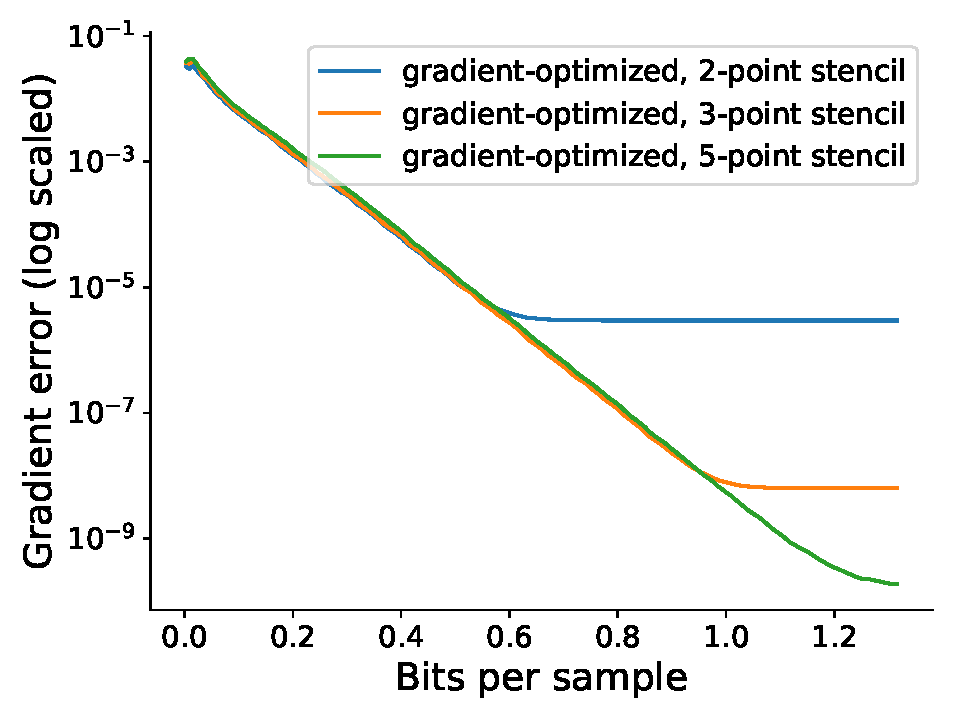
\includegraphics[width=0.48\linewidth]{img/gradient-laplacian/sine-gradient-stencils-full.pdf}}
	\subcaptionbox{zoomed in}
	{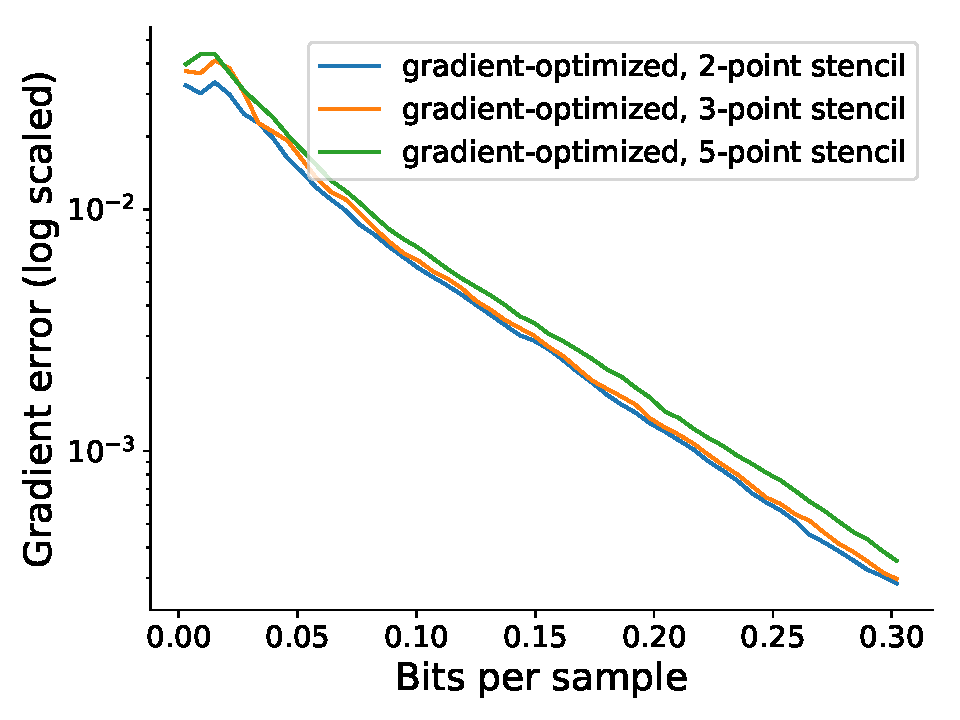
\includegraphics[width=0.48\linewidth]{img/gradient-laplacian/sine-gradient-stencils-cutoff.pdf}}
	\caption{Gradient error by three \emph{gradient-optimized} optimized streams on a sinusoid field,
	using different stencils. Smaller is better. The right plot zooms in on beginning part of the
	left plot, to better distinguish the curves. Smaller stencils perform marginally better than
	large stencils at low bit rates, but, unsurprisingly fail to track the ground-truth gradient at
	high bit rates.}
  \label{fig:gradient-error-comparison-stencils}
\end{figure}

\begin{figure}
	\centering
	\subcaptionbox{boiler}
	{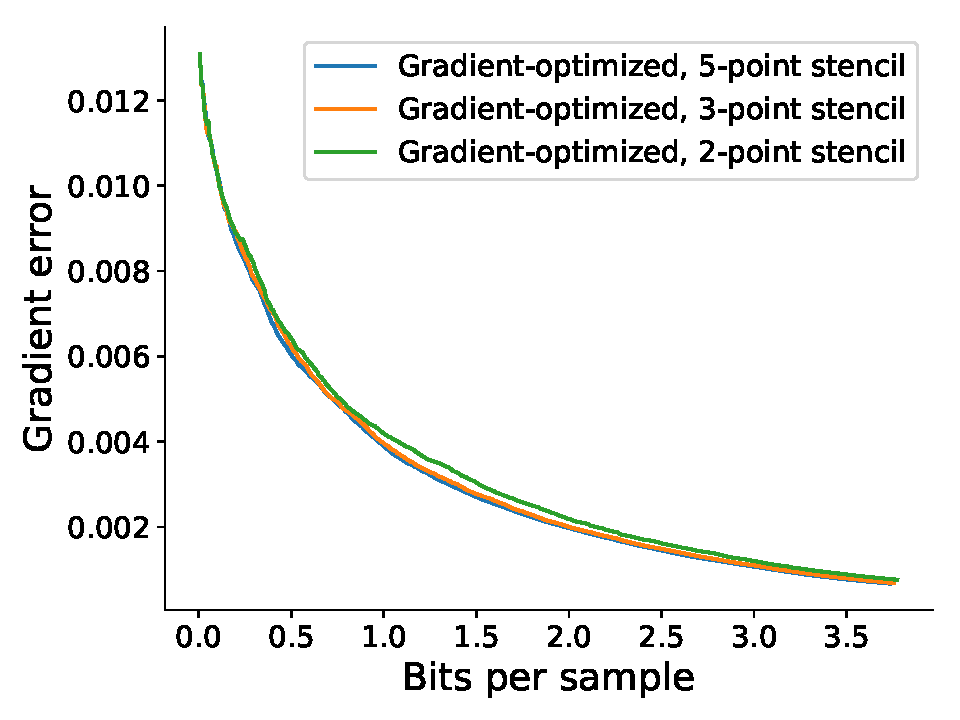
\includegraphics[width=0.48\linewidth]{img/gradient/compare-stencils/gradient-optimized-boiler.pdf}}
	\subcaptionbox{diffusivity}
	{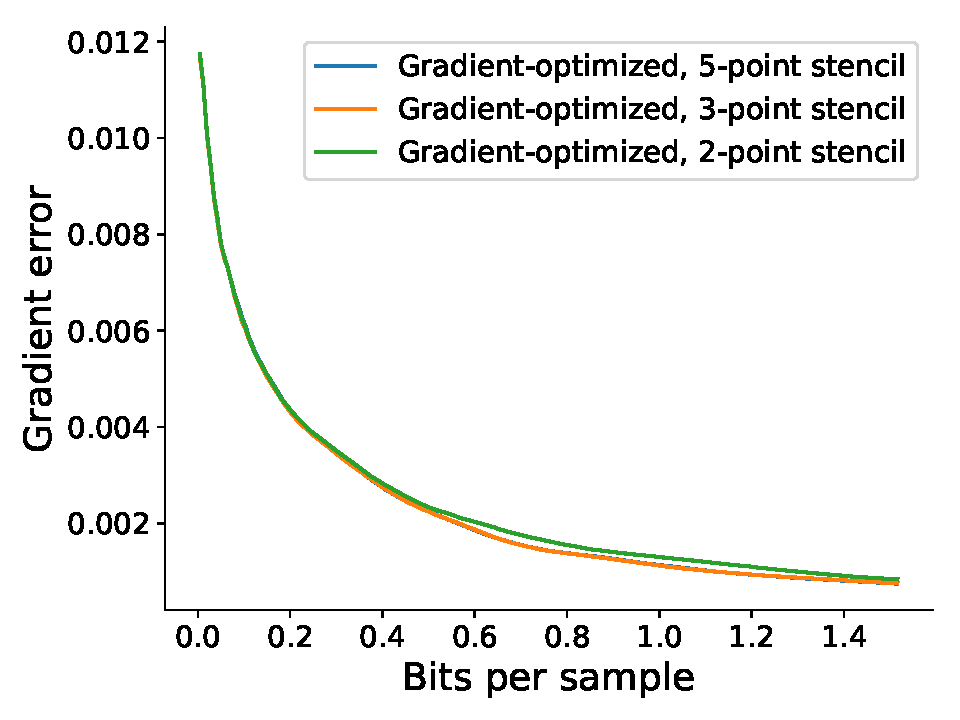
\includegraphics[width=0.48\linewidth]{img/gradient/compare-stencils/gradient-optimized-diffusivity.pdf}}
	\subcaptionbox{euler}
	{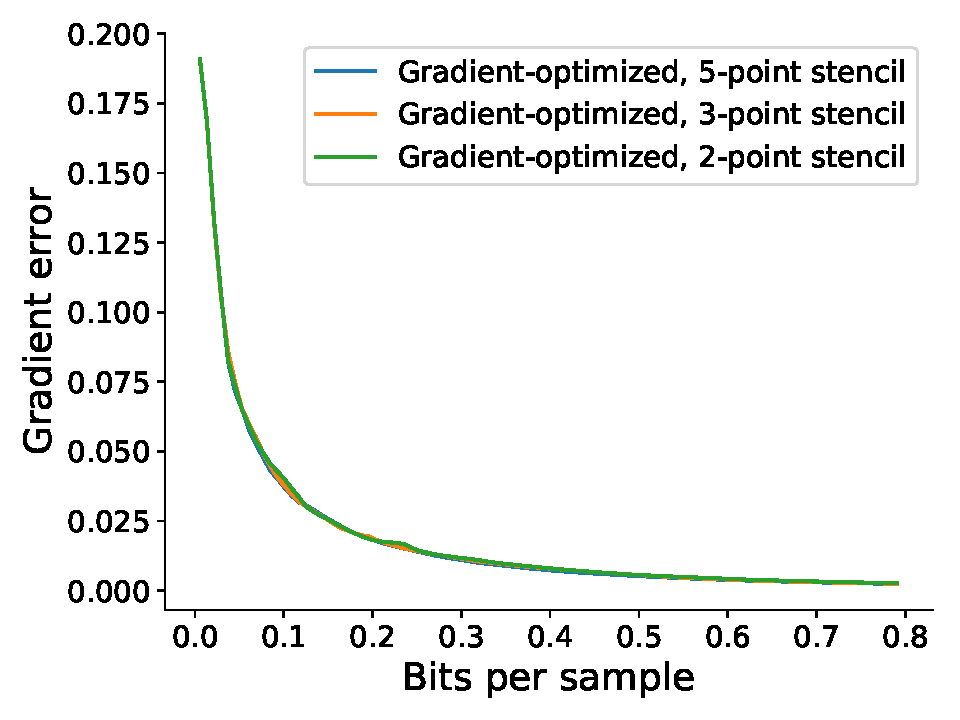
\includegraphics[width=0.48\linewidth]{img/gradient/compare-stencils/gradient-optimized-euler.pdf}}
	\subcaptionbox{pressure}
	{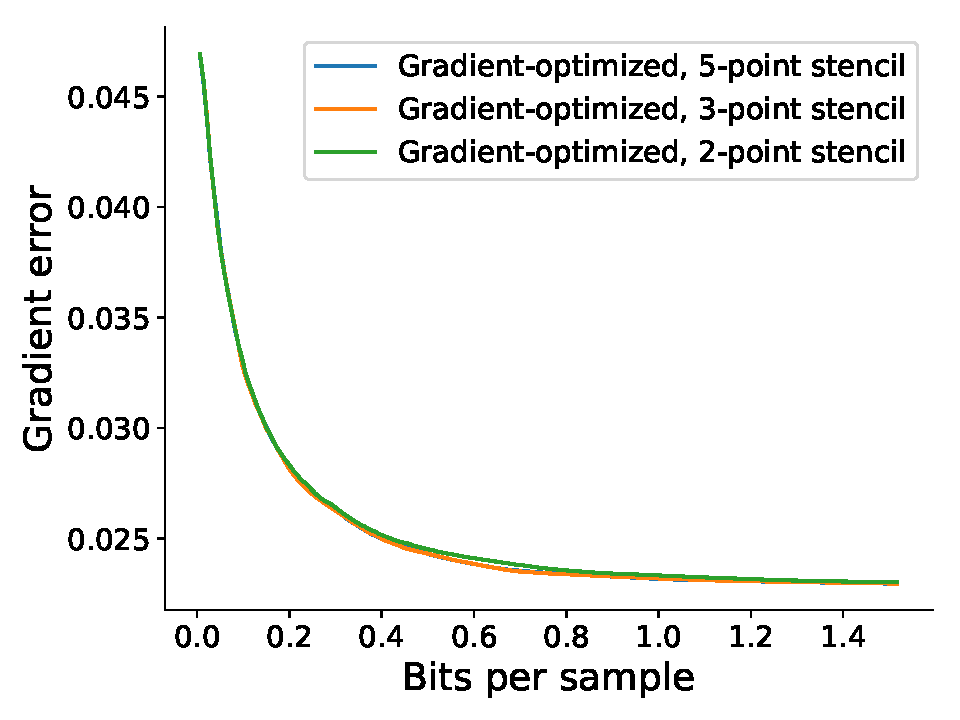
\includegraphics[width=0.48\linewidth]{img/gradient/compare-stencils/gradient-optimized-pressure.pdf}}
	\subcaptionbox{marschner-lobb}
	{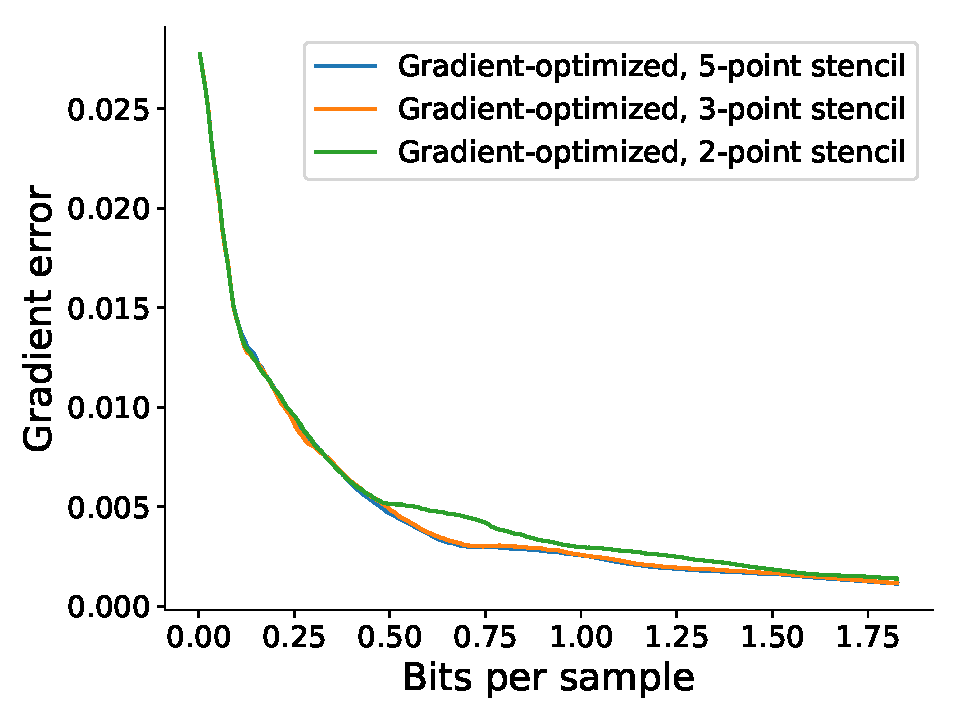
\includegraphics[width=0.48\linewidth]{img/gradient/compare-stencils/gradient-optimized-marschner-lobb.pdf}}
	\subcaptionbox{velocityz}
	{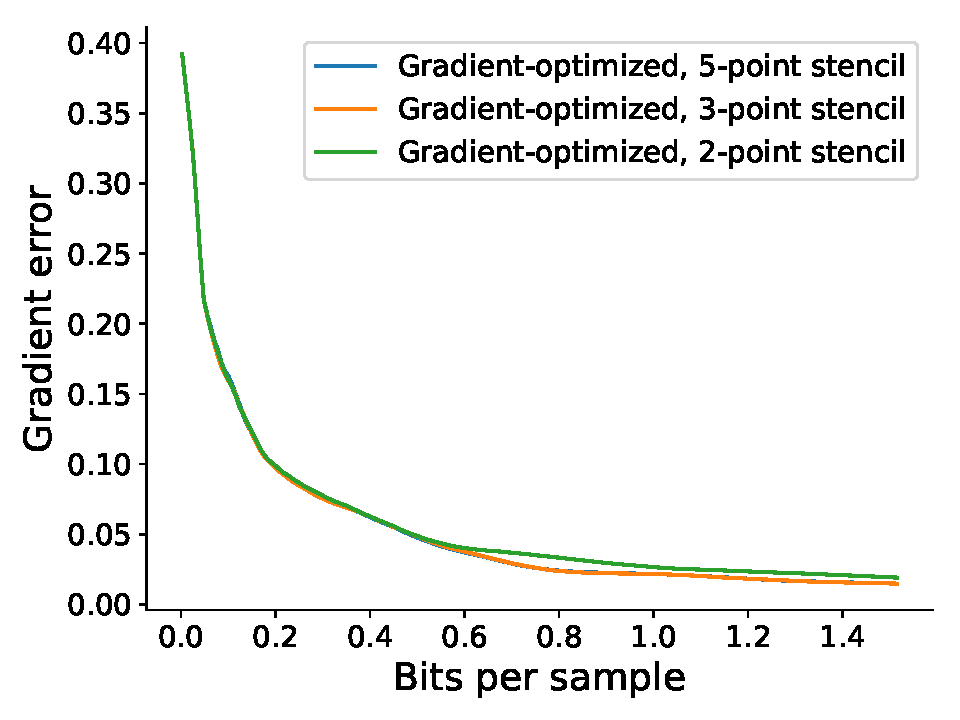
\includegraphics[width=0.48\linewidth]{img/gradient/compare-stencils/gradient-optimized-velocityz.pdf}}
	\caption{Gradient error for different stencil sizes, assuming the groundtruth gradient is computed
	using 5-point finite difference on the original field. There are no meaningful differences among
	the different stencil sizes.}
	\label{fig:gradient-error-comparison}
\end{figure}

\begin{figure}
	\centering
	\subcaptionbox{by wavelet norm}
	{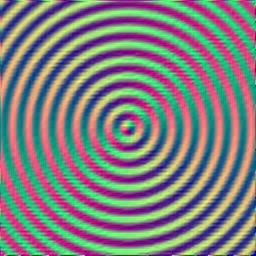
\includegraphics[width=0.49\linewidth]{img/gradient/gradient_0.png}}
	\subcaptionbox{by bit plane}
	{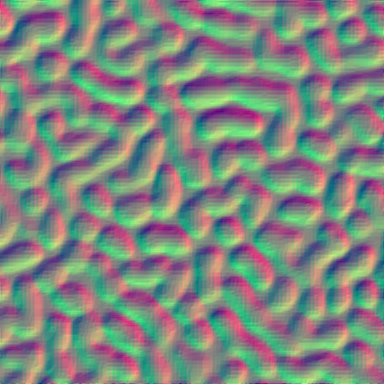
\includegraphics[width=0.49\linewidth]{img/gradient/gradient_1.png}}
	\subcaptionbox{gradient signature}
	{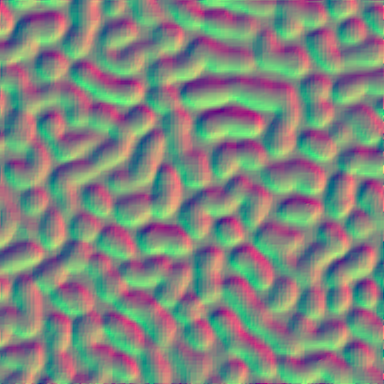
\includegraphics[width=0.49\linewidth]{img/gradient/gradient_2.png}}
	\subcaptionbox{groundtruth}
	{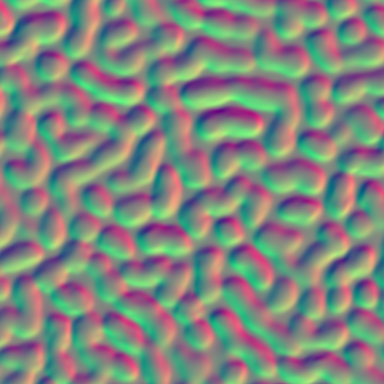
\includegraphics[width=0.49\linewidth]{img/gradient/groundtruth_gradient_0.png}}
	\caption{Comparison of reconstructed gradient fields among \emph{by wavelet norm}, \emph{by bit
	plane} and \emph{gradient signature} streams, for the \emph{marschner-lobb} function, at 0.52 bps.
	The \emph{by bit plane} and \emph{gradient signature} stream produces a gradient field with fewer
	artifacts.}
  \label{fig:gradient-rendering}
\end{figure}

When comparing the \emph{gradient-optimized}, \emph{rmse-optimized} streams as well as their
data-independent analogues, \emph{gradient signature} and \emph{by wavelet norm} (Figure
\ref{fig:gradient-error-comparison}), we see that in the {fig:gradient-error-comparison} compares
the \emph{gradient-optimized} with the \emph{rmse-optimized} streams for four data sets.

\begin{figure}
	\centering
	\subcaptionbox{boiler, 5-point stencil}
	{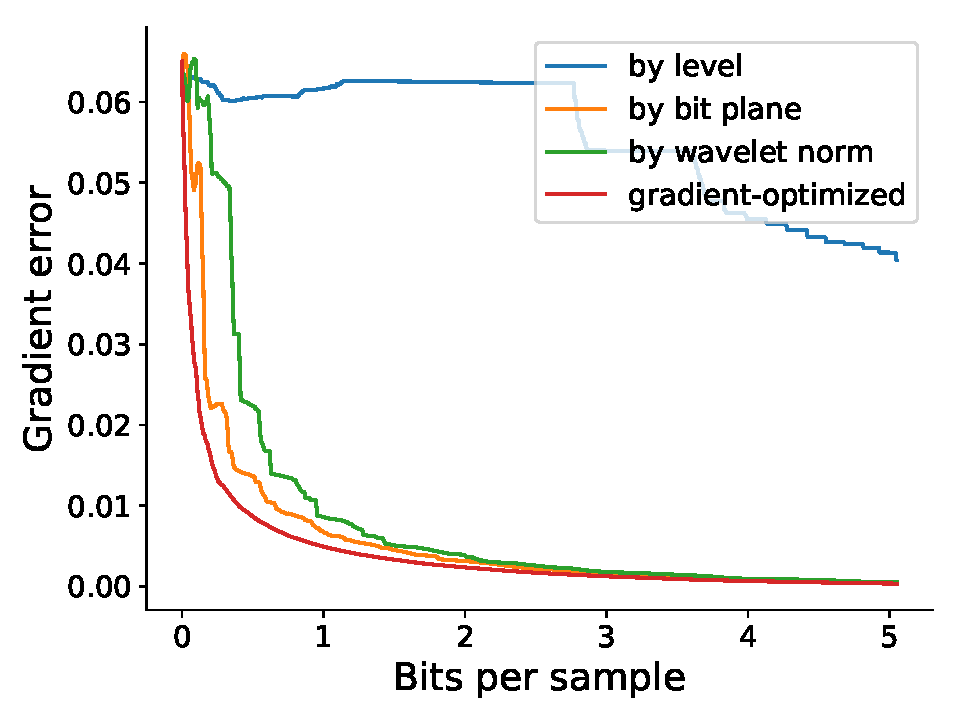
\includegraphics[width=0.48\linewidth]{img/gradient/5points/gradient-optimized-boiler.pdf}}
	\subcaptionbox{diffusivity, 5-point stencil}
	{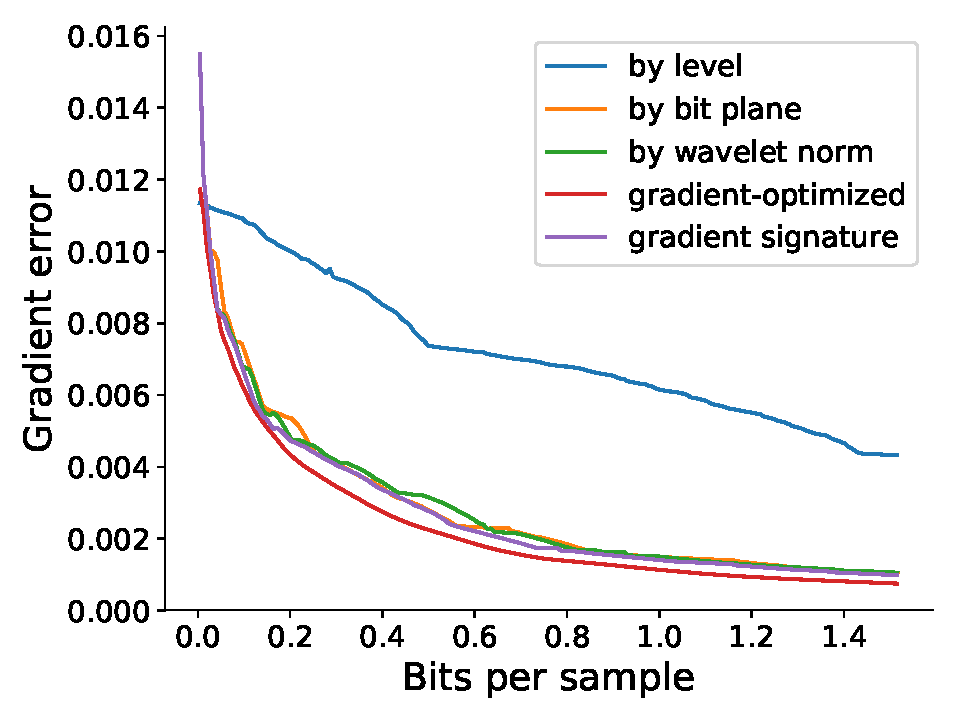
\includegraphics[width=0.48\linewidth]{img/gradient/5points/gradient-optimized-diffusivity.pdf}}
	\subcaptionbox{euler, 5-point stencil}
	{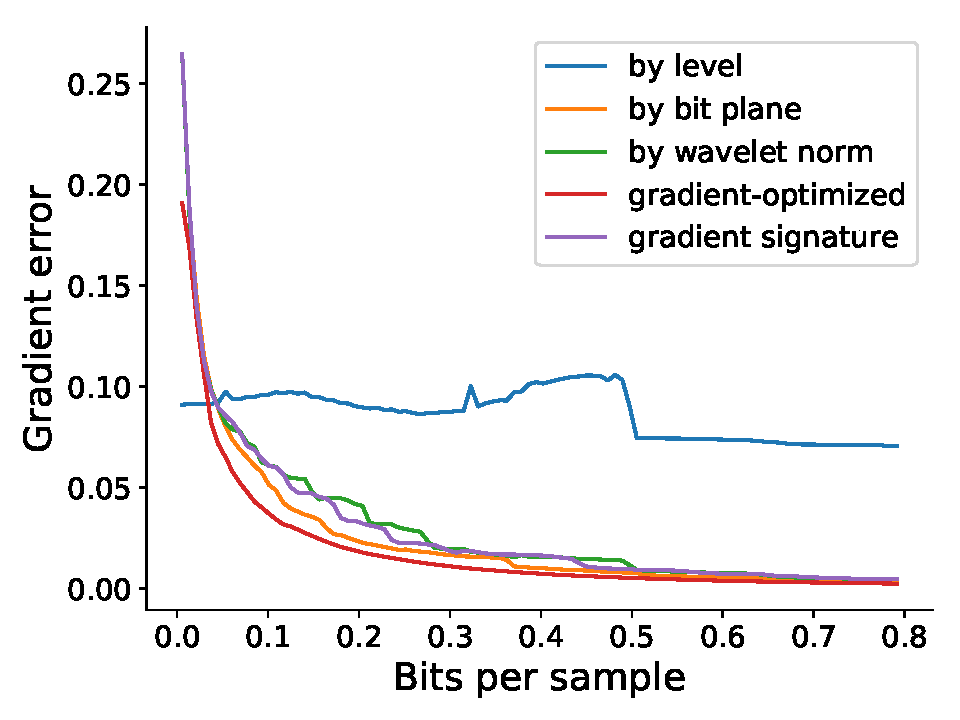
\includegraphics[width=0.48\linewidth]{img/gradient/5points/gradient-optimized-euler.pdf}}
	\subcaptionbox{pressure, 5-point stencil}
	{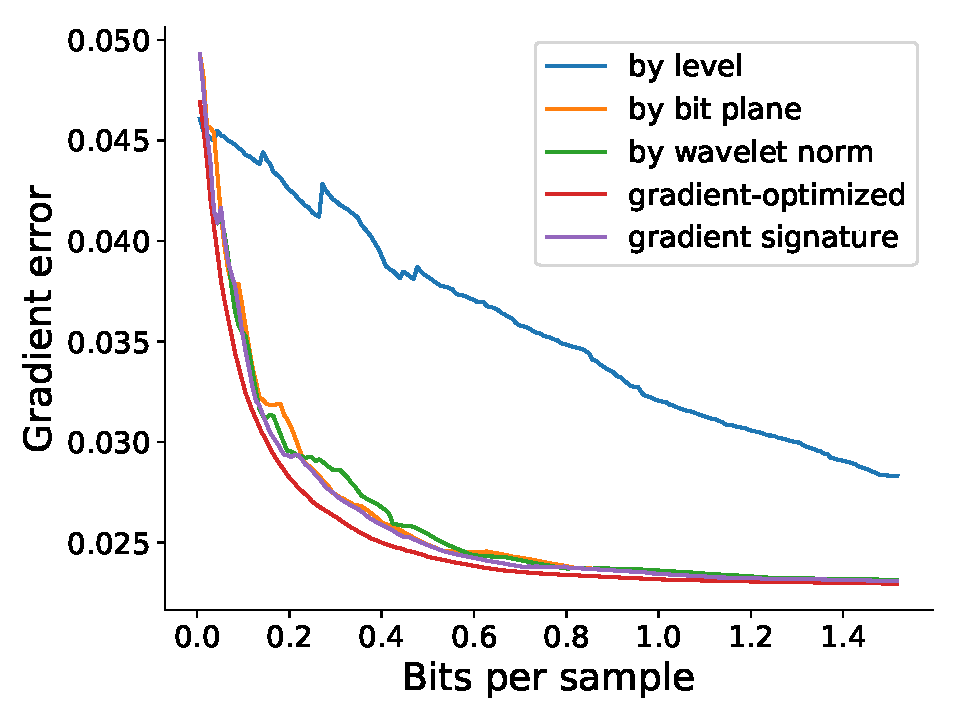
\includegraphics[width=0.48\linewidth]{img/gradient/5points/gradient-optimized-pressure.pdf}}
	\subcaptionbox{marschner-lobb, 5-point stencil}
	{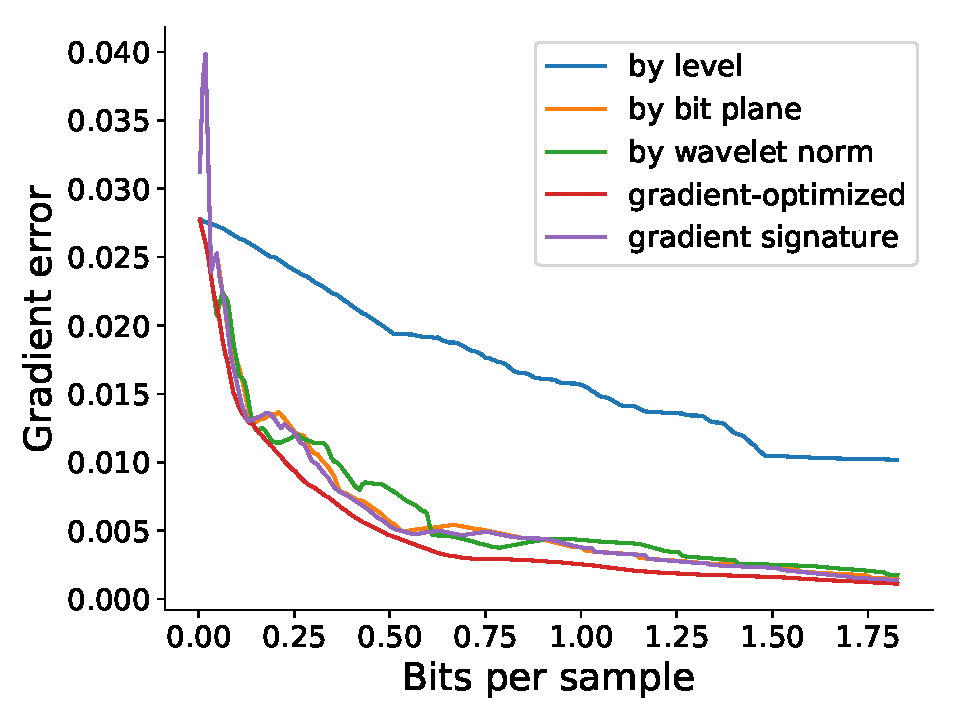
\includegraphics[width=0.48\linewidth]{img/gradient/5points/gradient-optimized-marschner-lobb.pdf}}
	\subcaptionbox{velocityz, 5-point stencil}
	{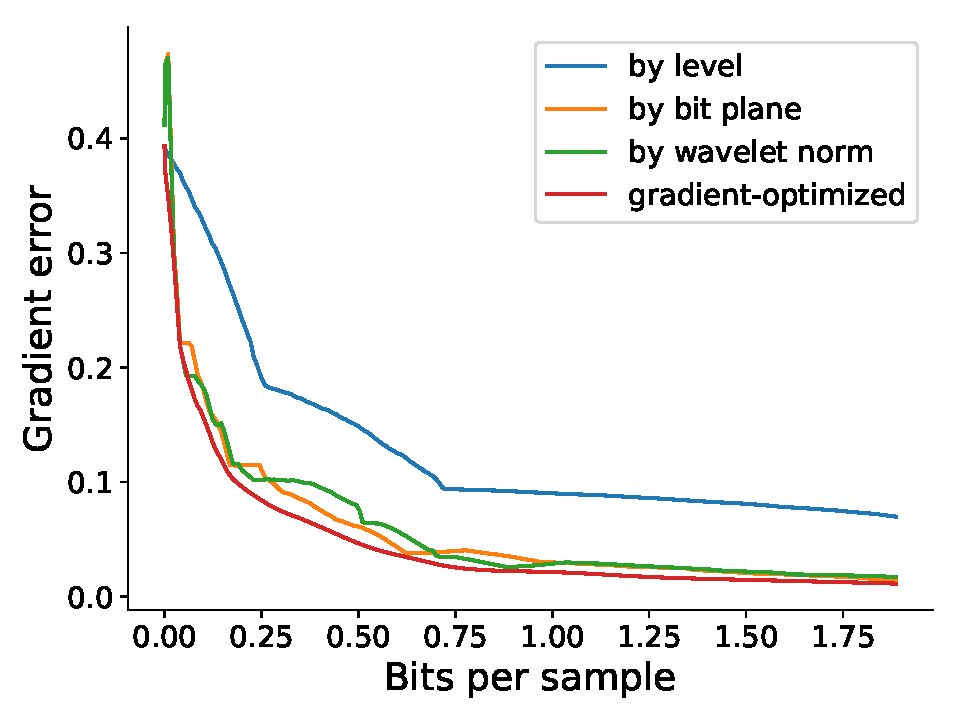
\includegraphics[width=0.48\linewidth]{img/gradient/5points/gradient-optimized-velocityz.pdf}}
	\caption{Gradient error comparison between \emph{gradient-optimized}, \emph{rmse-optimized},
	\emph{by wavelet norm}, and \emph{gradient signature} streams for four data sets, using the
	3-point stencil (left) and the 5-point stencil (right). Smaller is better. Chunks consisting of
	leading zero bits are removed from all streams. It all cases, the \emph{gradient-optimized} and
	\emph{rmse-optimized} streams perform the same, while \emph{gradient} signature is only slightly
	better than \emph{by wavelet norm}.}
	\label{fig:gradient-error-comparison}
\end{figure}

Figure \ref{fig:gradient-error-comparison} suggests that the \emph{rmse-optimized} streams are also
nearly optimal for gradient computation. The gradient operator is not invertible, that is, there are
infinitely many functions that result in the same gradient field. It is therefore not surprising
that the two streams both produce the best possible gradient progression. The \emph{rmse-optimized},
however, also produces an accurate function in addition to its gradient. We give evidence to this
claim is in Figure \ref{fig:gradient-comparison}, in which we reconstruct the euler data at $0.25$
bits per sample using both streams, and show the difference in gradient between the two. The two
gradient fields differ the most along very sharp edges, but are in general congruent (a), while the
\emph{rmse-optimized} stream produces significantly more accurate reconstruction of the function
itself (b, c, and d). It is therefore reasonable in practice to simply use \emph{by wavelet norm}
for the purpose of gradient computation.

\begin{figure}
	\centering
	\subcaptionbox{gradient difference}
	{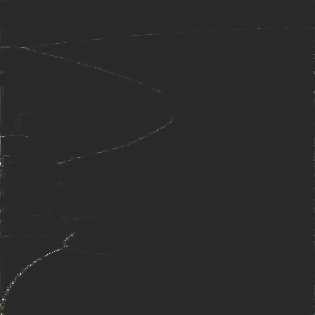
\includegraphics[width=0.24\linewidth]{img/gradient-laplacian/grad-diff.png}}
	\subcaptionbox{original data}
	{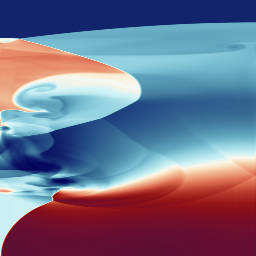
\includegraphics[width=0.24\linewidth]{img/gradient-laplacian/euler-original.png}}
	\subcaptionbox{\emph{rmse-optimized}}
	{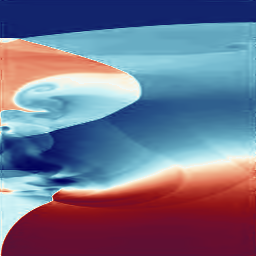
\includegraphics[width=0.24\linewidth]{img/gradient-laplacian/euler-rmse.png}}
	\subcaptionbox{\emph{gradient-optimized}, 3-point stencil}
	{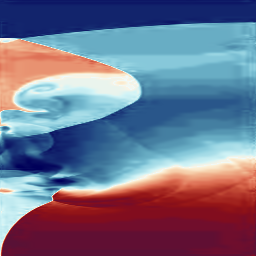
\includegraphics[width=0.24\linewidth]{img/gradient-laplacian/euler-gradient.png}}
	\caption{TODO: replace this figure (use 32-bit instead of 16-bit quantization). Comparing
	\emph{rmse-optimized} and \emph{gradient-optimized} at 0.25 bits per sample. }
	\label{fig:gradient-comparison}
\end{figure}

\subsection{Laplacian}

For Laplacian, we use the three-point finite difference in each dimension separately:
$\frac{{\partial}^2}{\partial{x^2}}f(x,y) \approx f(x-1,y)-2f(x,y)+f(x+1,y)$, and $\Delta
f=(\frac{{\partial}^2}{\partial{x^2}}+\frac{{\partial}^2}{\partial{y^2}})f$. The Laplacian error is
defined as the RMSE between the reconstructed Laplacian scalar field and the original Laplacian
scalar field. Again, algorithm [REF] is used to compute a \emph{laplacian-optimized} bit stream that
minimizes this error. In Figure \ref{fig:laplacian-comparison} we compare this stream with the
\emph{rmse-optimized} stream using the PSNR of the difference in Laplacian (compared to the
ground truth) as the error metric. The stream labeled \emph{laplacian signature} is to be ignored for
now. (TODO: why is it in the plot? maybe do not mention it at all? or just say that it will be explained later)

\begin{figure}
	\centering
	\subcaptionbox{boiler, 5-point stencil}
	{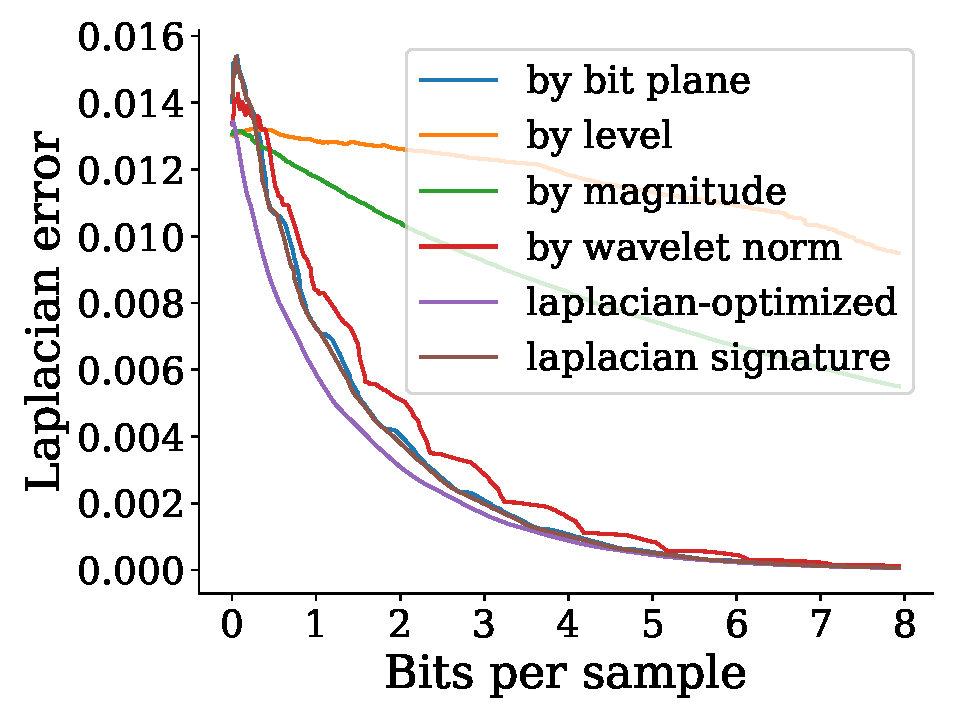
\includegraphics[width=0.48\linewidth]{img/laplacian/laplacian-optimized-boiler.pdf}}
	\subcaptionbox{diffusivity, 5-point stencil}
	{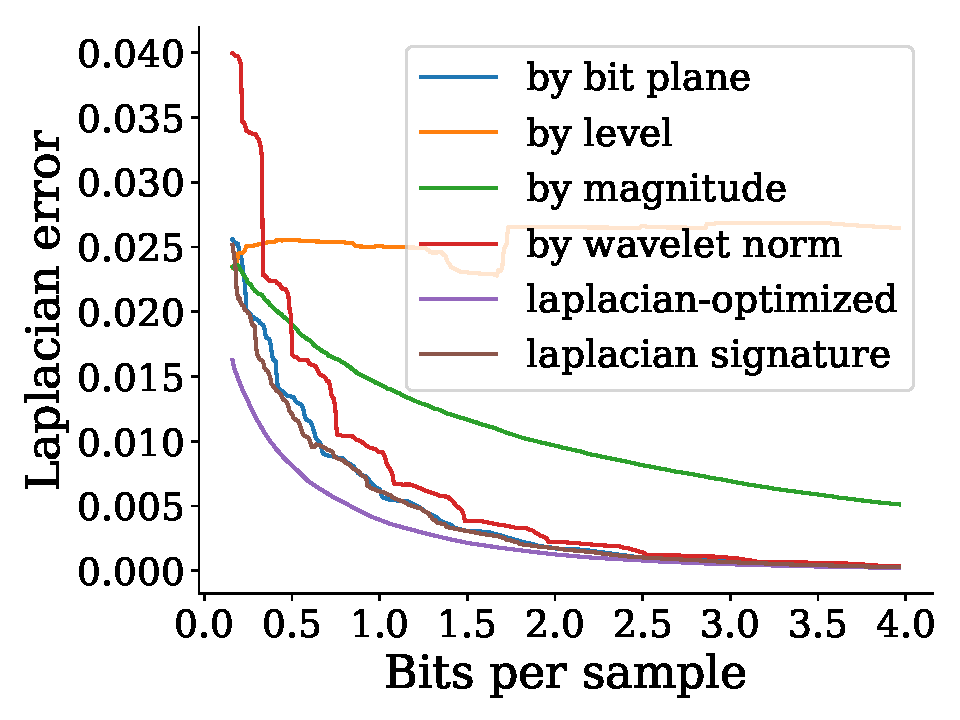
\includegraphics[width=0.48\linewidth]{img/laplacian/laplacian-optimized-diffusivity.pdf}}
	\subcaptionbox{euler, 5-point stencil}
	{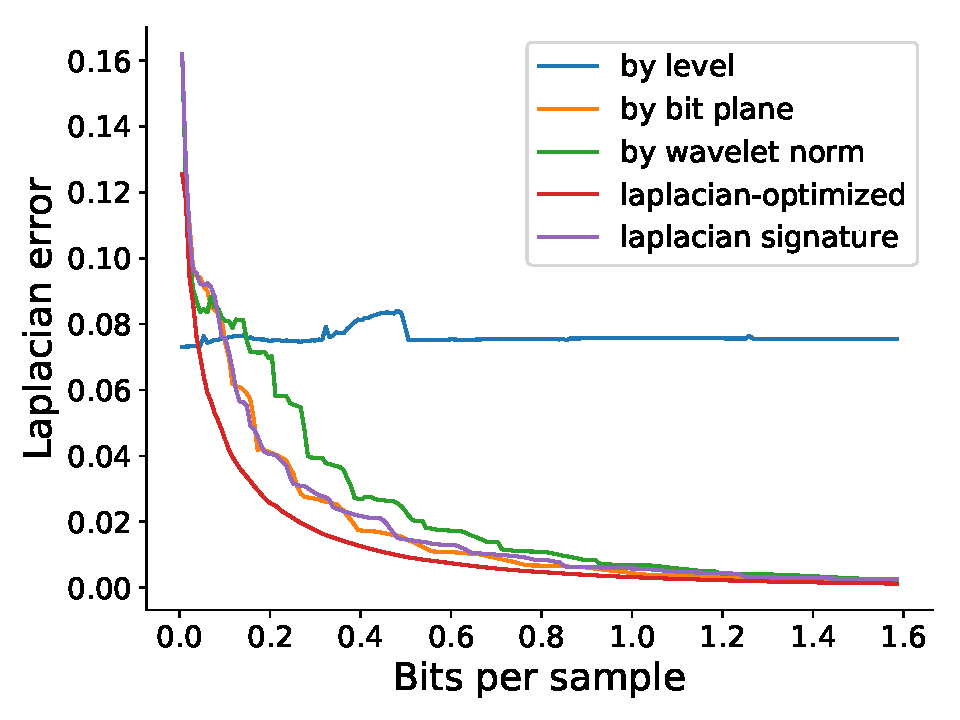
\includegraphics[width=0.48\linewidth]{img/laplacian/laplacian-optimized-euler.pdf}}
	\subcaptionbox{pressure, 5-point stencil}
	{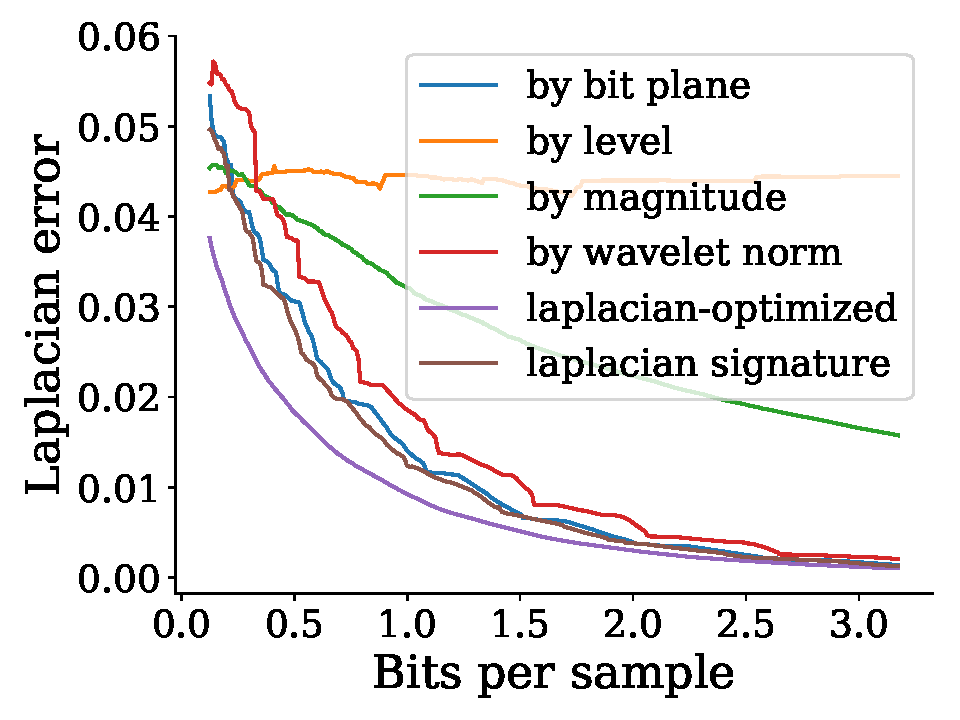
\includegraphics[width=0.48\linewidth]{img/laplacian/laplacian-optimized-pressure.pdf}}
	\subcaptionbox{marschner-lobb, 5-point stencil}
	{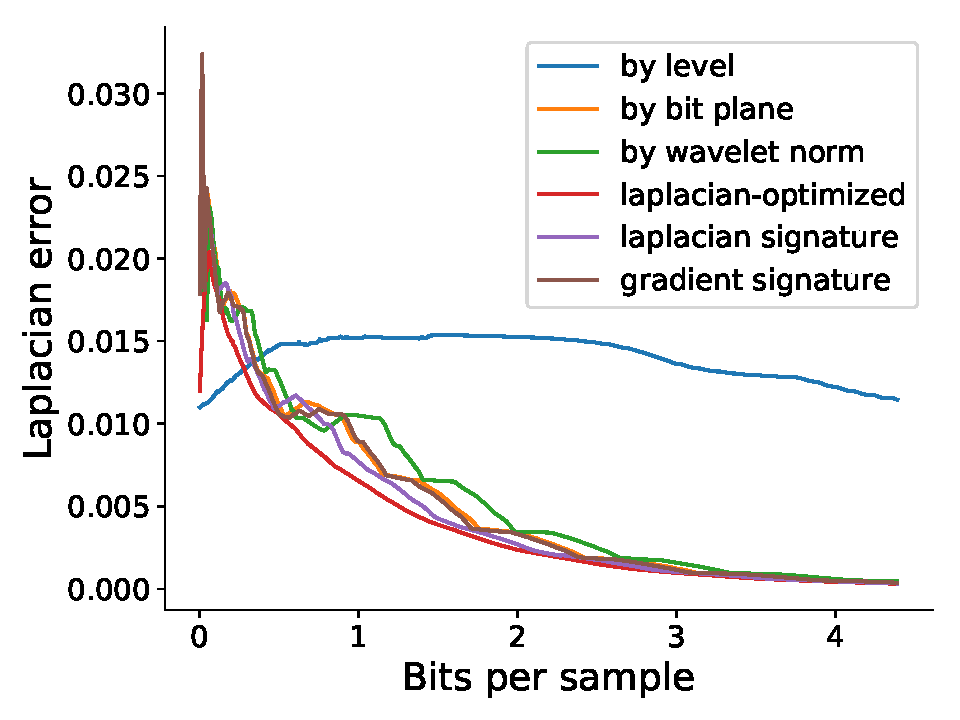
\includegraphics[width=0.48\linewidth]{img/laplacian/laplacian-optimized-marschner-lobb.pdf}}
	\subcaptionbox{velocityz, 5-point stencil}
	{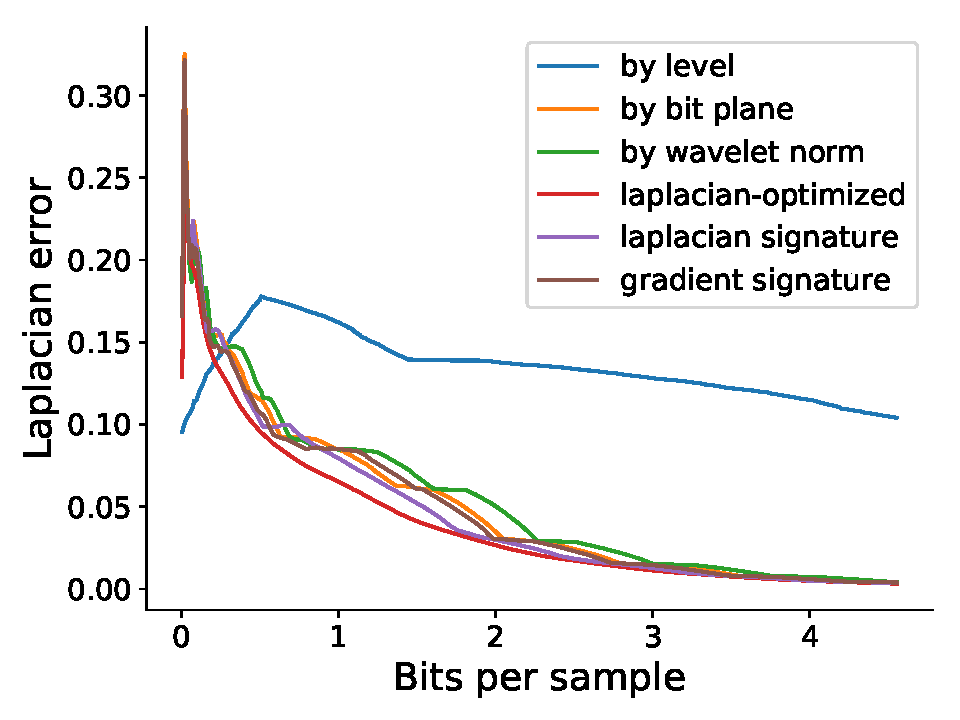
\includegraphics[width=0.48\linewidth]{img/laplacian/laplacian-optimized-velocityz.pdf}}
	\caption{Laplacian error}
	\label{fig:gradient-error-comparison}
\end{figure}

It can be observed that unlike the case for gradient, there exists significant differences between
the \emph{rmse-optimized} and \emph{laplacian-optimized} streams with regards. To understand these
differences we plot the precision of every wavelet coefficients at a low bit rate in Figure
\ref{fig:laplacian-precision-comparison} (a and b). When cross refererencing this Figure with Figure
\ref{fig:gradient-comparison}b we see that the \emph{laplacian-optimized} stream priotizes
finer-resolution bits where the sharp shockwave is, unlike the \emph{rmse-optimized} stream which
prefers lower-ordered, coarse-resolution bits. This effect makes sense intuitively, as the
derivative operator makes functions less smooth, hence amplifing hard edges. This happens in the
gradient case too, but to a much lesser degree.

\begin{figure}
	\centering
	\subcaptionbox{\emph{by wavelet norm}}
	{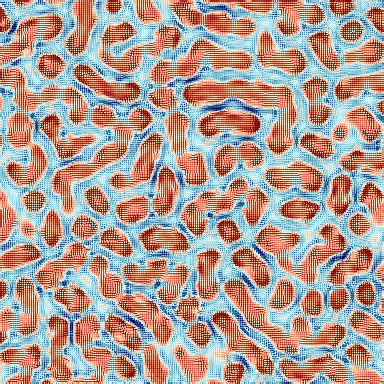
\includegraphics[width=0.48\linewidth]{img/laplacian/laplacian_0.png}}
	\subcaptionbox{\emph{by bit plane}}
	{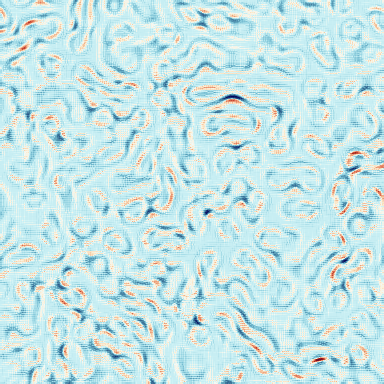
\includegraphics[width=0.48\linewidth]{img/laplacian/laplacian_1.png}}
	\subcaptionbox{\emph{laplacian signature}}
	{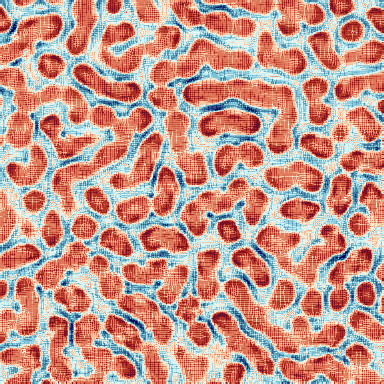
\includegraphics[width=0.48\linewidth]{img/laplacian/laplacian_2.png}}
	\subcaptionbox{\emph{groundtruth}}
	{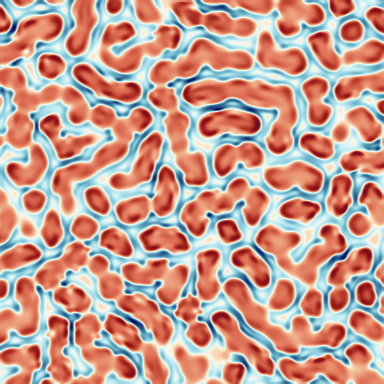
\includegraphics[width=0.48\linewidth]{img/laplacian/groundtruth_laplacian_0.png}}
	\caption{Laplacian rendering, diffusivity}
	\label{fig:laplacian-precision-comparison}
\end{figure}

\begin{figure}
	\centering
	\subcaptionbox{\emph{by wavelet norm}}
	{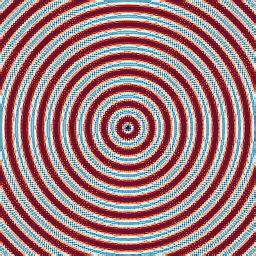
\includegraphics[width=0.48\linewidth]{img/laplacian/laplacian_00.png}}
	\subcaptionbox{\emph{by bit plane}}
	{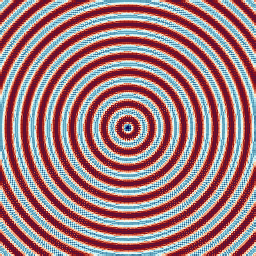
\includegraphics[width=0.48\linewidth]{img/laplacian/laplacian_11.png}}
	\subcaptionbox{\emph{laplacian signature}}
	{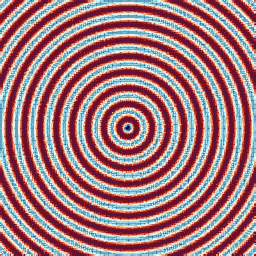
\includegraphics[width=0.48\linewidth]{img/laplacian/laplacian_22.png}}
	\subcaptionbox{\emph{groundtruth}}
	{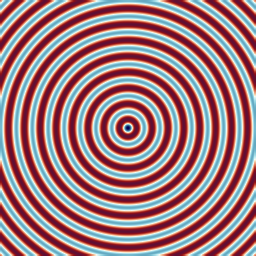
\includegraphics[width=0.48\linewidth]{img/laplacian/groundtruth_laplacian_00.png}}
	\caption{Laplacian rendering, marschner-lobb}
	\label{fig:laplacian-precision-comparison}
\end{figure}

\begin{figure}
	\centering
	\subcaptionbox{\emph{laplacian-optimized}}
	{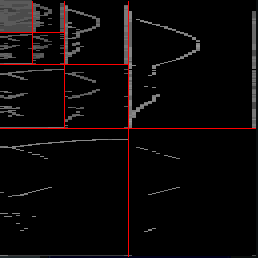
\includegraphics[width=0.32\linewidth]{img/gradient-laplacian/euler-prec-lap.png}}
	\subcaptionbox{\emph{rmse-optimized}}
	{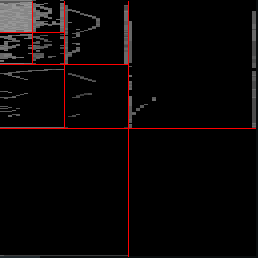
\includegraphics[width=0.32\linewidth]{img/gradient-laplacian/euler-prec-rmse.png}}
	\subcaptionbox{\emph{laplacian signature}}
	{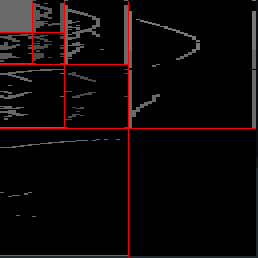
\includegraphics[width=0.32\linewidth]{img/gradient-laplacian/euler-prec-signature.png}}
	\caption{Precision distribution of wavelet coefficients at 0.25 bits per sample for the euler data
	set. Each square box with red boundary is a wavelet subband (the coarsest subband is in the top
	left). Brighter pixels correspond to higher-precision wavelet coefficients (black means no bit of
	that coefficient has not been received, while white means the whole coefficient has been
	received).}
	\label{fig:laplacian-precision-comparison}
\end{figure}

\emph{rmse-optimized}, \emph{laplacian-optimized}, and also \emph{gradient-optimized} for the euler
data set are visualized in Figure \ref{fig:signature-comparison}. 

\begin{figure}
	\centering
	\subcaptionbox{\emph{rmse-optimized}}
	{
\includegraphics[width=0.32\linewidth]{img/gradient-laplacian/SIG-GREEDY-(rmse).png}}
	\subcaptionbox{\emph{laplacian-optimized}}
	{
\includegraphics[width=0.32\linewidth]{img/gradient-laplacian/SIG-GREEDY-(laplacian).png}}
	\subcaptionbox{\emph{gradient-optimized}}
	{
\includegraphics[width=0.32\linewidth]{img/gradient-laplacian/SIG-GREEDY-(gradient).png}}
	\caption{Stream signatures visualized through a linear-blue color map (brighter is higher
	priority). From left to right: higher-ordered to lower-ordered bit planes. From top to bottom:
	coarser to finer subbands. Note that the streams from which the signatures are extracted do not
	contain leading zero bits, which explains the very dark cells }
	\label{fig:signature-comparison}
\end{figure}

Using the signature for \emph{laplacian-optimized}, we are able construct a data-independent stream
(in the sense that once the signature is computed and is given, the ordering of the bits follows the
the signature only). This stream, called \emph{laplacian signature}, performs at least as well as,
and often better, than \emph{rmse-optimized} for all data sets (see Figure
\ref{fig:laplacian-comparison}). The reason \emph{laplacian signature} does not always outperform
\emph{rmse-optimized}, and that there is still a gap between itself and \emph{laplacian-optimized}
is that the signature is computed essentially by `'averaging'' local signatures, a process that
lessen the effectiveness of the signature when the data is highly inhomogenous (e.g., the euler data
set with its sharp shockwaves). Nevertheless, even with one signature for the whole domain, we are
able to reconstruct more accurate Laplacian in all cases in experiment. In practice, the signature
is a tiny piece of meta information that can be pre-computed, stored, and transmitted before any
value bits to help `'steer'' the data stream, whenever Laplacian is the quantity of interest.
